\section{Application Implementation}
This section will describe the implementation of the study application, mostly regarding how data was collected, how features were computed as well as how the data was sent to a Firebase instance. The study app used the package while it was in an earlier iteration. In this iteration almost none of the logic related to storing and loading data was part of the package, and as such all of this had to be written in the application instead. This section will provide source code examples of how the application should be implemented with the new API, since the old version is deprecated. Largely, the data flow of the study app has not changed but the concrete implementation has, in the sense that much fewer lines of code are needed.

\subsection{Architecture Overview}
To provide a high level overview of the different components which make up the study application, a component diagram displayed in Figure \ref{fig:app-component-diagram}. The MobilityStudy component in blue is the component responsible for managing the application state but does not do much outside of this since the application state management required is minimal. Had it been a more complex application with many different screens and a state which had to be maintained across these screens (for example a shopping cart in a shopping app) then more logic would lie inside the MobilityStudy component. Instead the Main Screen is spawned from the MobilityStudy component which in turn creates an AppProcessor instance. The AppProcessor instance is responsible for a multitude of tasks, such as asking for permissions, collection location data, and computing features. Storing and loading from the disk is done through the FileManager component which includes location data, Stops, Moves, MobilityContexts and diary answers. This component is also responsible for uploading the stored data to Firebase.

\begin{figure}
    \centering
    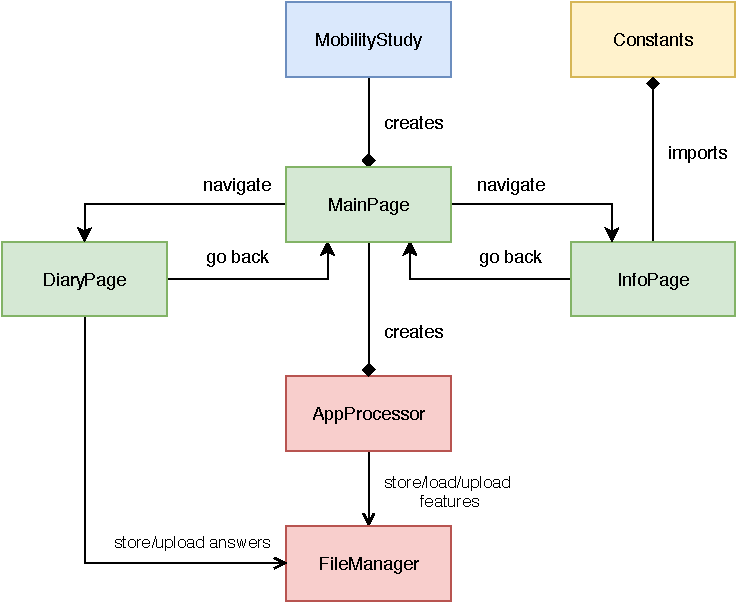
\includegraphics[width=\textwidth]{images/diagrams/app-diagram.pdf}
    \caption{Component diagram for the study application displaying the different building blocks and the interactions between them}
    \label{fig:app-component-diagram}
\end{figure}

\subsection{Diary Implementation}

\subsection{Firebase Storage}

\subsection{Firebase Cloud Messaging}


\subsection{Asynchronous Computation and Threading}
One concept not discussed much so far is the need for asynchronous computation and the use of multi-threading. Flutter applications support multi-threading, which means a main thread runs the user interface, and background threads can be spawned in order to perform heavy computation which would otherwise 'clog' the main thread, which means the user will experience a frozen UI. In the study app there was no real user interface so to speak, but in a real-world application there will be a user interface which cannot be allowed to freeze due to the feature calculation. In Flutter threads are referred to as Isolates which communicate using a \textit{SendPort} and a \textit{ReceivePort}. These two objects can be used to transfer other objects between threads, such that the main thread can request a background thread to calculate the features, and the background thread will then send back a \textit{MobilityContext} object once finished. 

\begin{minted}{dart}
Future<MobilityContext> _computeFeaturesAsync() async {
  ReceivePort receivePort = ReceivePort();
  await Isolate.spawn(_asyncComputation, receivePort.sendPort);
  SendPort sendPort = await receivePort.first;

  MobilityContext mobilityContext = await _relay(sendPort);
  return mobilityContext;
}
\end{minted}

The \verb|_relay| method works as an interface between the \verb|_computeFeaturesAsync| method which runs on the UI thread and the static method \verb|_asyncComputation| which runs on the background thread and simply relays messages between the two threads.

\begin{minted}{dart}
Future _relay(SendPort sendPort) {
  ReceivePort receivePort = ReceivePort();
  sendPort.send([receivePort.sendPort]);
  return receivePort.first;
}
\end{minted}

Lastly, the \verb|_asyncComputation| method is static which is due to the computation being done in a separate thread than than the main thread. If the objects contained within the \textit{AppProcessor} instance (i.e. in the main thread) were to change their state while computation was ongoing in the background thread, then the resulting computation would produce an outdated result. The \textit{ContextGenerator} is also a static class without mutable state and can therefore be used to compute the Mobility Context without the need for mutable state anywhere in the chain, once the message reaches the background thread.

\begin{minted}{dart}
static void _asyncComputation(SendPort sendPort) async {
  ReceivePort receivePort = ReceivePort();
  sendPort.send(receivePort.sendPort);
  List args = await receivePort.first;
  SendPort replyPort = args[0];

  MobilityContext context =
      await ContextGenerator.generate(usePriorContexts: true);

  replyPort.send(context);
}
\end{minted}

